% Skip over this boring header down a bit
%%%%%%%%%%%%%%%%%%%%%%%%%%%%%%%%%%%%%%%%%%%%%%%%
\documentclass[usenames,dvipsnames,10pt,aspectratio=169]{beamer} 
% Add option 'aspectratio=169' for 16:9 widescreen 
% Add option  'handout' to ignore animations
% If you have a smaller amount of text, feel free to also try '11pt'! / Jesper

\usepackage[utf8]{inputenc}
\usepackage{verbatim}
\usepackage{minted}
\usemintedstyle{monokai}
\usepackage{graphicx}
\usepackage{wrapfig}
\usepackage[document]{ragged2e}
\usetheme{umu}

\usepackage{hyperref}
\hypersetup{
    colorlinks=true,
    linkcolor=ucuyellow,
    filecolor=ucuyellow,      
    urlcolor=ucuyellow,
}
\urlstyle{same}

\usepackage[shortlabels]{enumitem}

%%% Bibliography
\usepackage[style=authoryear,backend=biber]{biblatex}
\addbibresource{bibliography.bib}

\DeclareNameAlias{author}{given-family}

%%% Suppress biblatex annoying warning
\usepackage{silence}
\WarningFilter{biblatex}{Patching footnotes failed}

%%% Some useful commands
% pdf-friendly newline in links
\newcommand{\pdfnewline}{\texorpdfstring{\newline}{ }} 
% Fill the vertical space in a slide (to put text at the bottom)
\newcommand{\framefill}{\vskip0pt plus 1filll}

%%% Enter additional packages below 
\renewcommand{\proofname}{\sffamily{Proof}}

%%%%%%%%%%%%%%%%%%%%%%%%%%%%%%%%%%%%%%%%%%%%%%%%%%%%%%%%%%%%%%%%%%%%%%%%%%%%%%%%%%%%%
\title[Rust \#3]{Rust \#3: Collections,\\ \vspace{0.1cm}
Iterators, and Traits}
\author[Sultanov Andriy]{Sultanov Andriy}
\institute{APPS@UCU}

\begin{document}

\begin{frame}
\titlepage
\end{frame}

\begin{frame}{\contentsname}
\tableofcontents
\end{frame}

\framepic{graphics/1.jpg}{
 \textcolor{ucuwhite}{Collections in Rust}
 \vskip 0.5cm
 }

\section{Collections in Rust}

\begin{frame}{Collections}
	\framesubtitle{Most common collections}
	\large
	Rust's standard library implements some of\\
	the most common collections:
\begin{itemize}[label=$\bullet$]
	\item \textbf{Sequences}: \textcolor{ucuyellow}{String}, 
	\textcolor{ucuyellow}{Vec}, 
		\textcolor{ucuyellow}{VecDeque}, \textcolor{ucuyellow}{LinkedList}
	\item \textbf{Maps}: \textcolor{ucuyellow}{HashMap}, \textcolor{ucuyellow}{BTreeMap}
	\item \textbf{Sets}: \textcolor{ucuyellow}{HashSet}, \textcolor{ucuyellow}{BTreeSet}
	\item \textbf{Misc}: \textcolor{ucuyellow}{BinaryHeap}
\end{itemize}

	\vspace{0.4cm}
	In most cases, you are going to be fine with\\
	using just \textcolor{ucuyellow}{String}, \textcolor{ucuyellow}{Vec}, 
	\textcolor{ucuyellow}{HashMap}, \textcolor{ucuyellow}{HashSet}.
\end{frame}

\begin{frame}{Collections}
	\framesubtitle{String}
	\large
	Strings are dynamic (heap-allocated) UTF-8 collections!
	\vspace{0.3cm}
	\inputminted[fontsize=\large]{rust}{code/string.rs}
	\vspace{0.3cm}
\end{frame}

\begin{frame}{Collections}
	\framesubtitle{String}
	\large
	\inputminted[fontsize=\large]{rust}{code/string1.rs}
	\vspace{0.3cm}
\end{frame}

\begin{frame}{Collections}
	\framesubtitle{String}
	\large
	\inputminted[fontsize=\large]{rust}{code/string2.rs}
	\vspace{0.3cm}
\end{frame}

\begin{frame}{Collections}
	\framesubtitle{String}
	\large
	\inputminted[fontsize=\large]{rust}{code/string3.rs}
	\vspace{0.3cm}
\end{frame}

\begin{frame}{Collections}
	\framesubtitle{Vector}
	\large
	Vectors are your typical growable generic containers:
	\vspace{0.3cm}
	\inputminted[fontsize=\large]{rust}{code/vector.rs}
\end{frame}

\begin{frame}{Collections}
	\framesubtitle{Vector}
	\large
	\inputminted[fontsize=\normalsize]{rust}{code/vector1.rs}
	\vspace{0.3cm}
\end{frame}

\begin{frame}{Collections}
	\framesubtitle{HashMap}
	\large
	HashMap is a 'dictionary' type that's generic over <K, V>:
	\vspace{0.2cm}
	\inputminted[fontsize=\normalsize]{rust}{code/hashmap.rs}
\end{frame}

\begin{frame}{Collections}
	\framesubtitle{HashMap}
	\large
	\inputminted[fontsize=\large]{rust}{code/hashmap1.rs}
	\vspace{0.3cm}
\end{frame}

\begin{frame}{Collections}
	\framesubtitle{HashMap}
	\large
	\inputminted[fontsize=\Large]{rust}{code/hashmap2.rs}
	\vspace{0.3cm}
\end{frame}

\begin{frame}{Collections}
	\framesubtitle{HashSet}
	\large
	HashSet is a set that's generic over <T>:
	\vspace{0.2cm}
	\inputminted[fontsize=\normalsize]{rust}{code/hashset.rs}
\end{frame}

\begin{frame}{Collections}
	\framesubtitle{HashSet}
	\large
	\inputminted[fontsize=\large]{rust}{code/hashset1.rs}
\end{frame}

\framepic{graphics/1.jpg}{
	\textcolor{ucuwhite}{Generics and Traits}
 \vskip 0.5cm
 }

\section{Generics and Traits}

\begin{frame}{Generics}
	\framesubtitle{General}
	\Large
	Generics are a common way to generalize types and\\
	functionalities. This can reduce code duplication and\\
	allow for different and user-defined types to be\\
	used with generic functions.\\
	\vspace{0.4cm}
\end{frame}

\begin{frame}{Generics}
	\framesubtitle{Generic structs and enums}
	\large
	We've already seen a few examples of generic types\\
	in Rust (as opposed to concrete types): 
	\vspace{0.2cm}
	\inputminted[fontsize=\large]{rust}{code/generics1.rs}
\end{frame}

\begin{frame}{Generics}
	\framesubtitle{Generic structs and enums}
	Let's write one of these ourselves:
	\vspace{0.2cm}
	\inputminted[fontsize=\large]{rust}{code/generics2.rs}
\end{frame}

\begin{frame}{Generics}
	\framesubtitle{Generic structs and enums}
	\large
	We can also be more specific with \textcolor{ucuyellow}{impl} blocks:
	\vspace{0.2cm}
	\inputminted[fontsize=\large]{rust}{code/generics3.rs}
\end{frame}

\begin{frame}{Generics}
	\framesubtitle{Functions}
	\large
	In Rust, generics can be used in a lot of cases,\\
	let's first look at \textcolor{ucuyellow}{generic functions}.\\
	\vspace{0.2cm}
	Let's imagine we have two functions that are\\
	basically the same except for parameter types:\\
	\vspace{0.2cm}
	\inputminted[fontsize=\large]{rust}{code/generics4.rs}
\end{frame}

\begin{frame}{Generics}
	\framesubtitle{Functions}
	\large
	Let's rewrite these functions into a generic function:\\
	\vspace{0.2cm}
	\inputminted[fontsize=\Large]{rust}{code/generics5.rs}
	\vspace{0.2cm}
	This doesn't compile though...\\
\end{frame}

\begin{frame}{Traits}
	\framesubtitle{General}
	\large
	Rust, at compile-time, needs to be sure that you\\
	won't be able to call these functions with a type\\
	that won't have the needed functionality.\\
	\vspace{0.3cm}
	Rust has a concept that allows to tell the compiler\\
	about type's functionality, and to share that\\
	functionality between several types - \textcolor{ucuyellow}{traits}.\\
\end{frame}	

\begin{frame}{Traits}
	\framesubtitle{General}
	\large
	What's the type functionality? Basically - just the\\
	methods we can call on that type, and traits\\
	allow us to group those methods in specific sets.\\
	\vspace{0.4cm}
	Let's imagine we have several possible types of\\
	students - kindergarten, school and university\\
	students. We want to be able to get a report on\\
	them - with their names, grades etc.\\
\end{frame}

\begin{frame}{Traits}
	\framesubtitle{Example}
	\large
	We define an 'interface' of our shared functionality\\
	with method signatures without any implementation.\\
	We can also provide default functionality for a trait:\\
	\vspace{0.2cm}
	\inputminted[fontsize=\normalsize]{rust}{code/traits1.rs}
	\vspace{0.2cm}
\end{frame}

\begin{frame}{Traits}
	\framesubtitle{Example}
	\large
	Let's implement this trait for one of our student types:\\
	\vspace{0.2cm}
	\inputminted[fontsize=\normalsize]{rust}{code/traits2.rs}
\end{frame}

\begin{frame}{Traits}
	\framesubtitle{Traits as parameters}
	\large
	When we want to be sure that the type we take as a parameter\\
	has the needed functionality, we can use the \textcolor{ucuyellow}{impl Trait} syntax:\\
	\vspace{0.2cm}
	\inputminted[fontsize=\large]{rust}{code/traits3.rs}
\end{frame}

\begin{frame}{Traits}
	\framesubtitle{Traits as parameters}
	\large
	We can also specify having multiple traits\\
	implemented as a requirement:\\
	\vspace{0.2cm}
	\inputminted[fontsize=\large]{rust}{code/traits4.rs}
\end{frame}

\begin{frame}{Traits}
	\framesubtitle{Traits as parameters}
	\large
	If your function is generic over several types with\\
	different trait bounds, it's better to use \textcolor{ucuyellow}{where} syntax:\\	
	\vspace{0.2cm}
	\inputminted[fontsize=\large]{rust}{code/traits5.rs}
\end{frame}

\begin{frame}{Generics and Traits}
	\framesubtitle{Bounds}
	\large
	Let's return to an earlier example of a generic function:
	\vspace{0.2cm}
	\inputminted[fontsize=\Large]{rust}{code/generics5.rs}
	\vspace{0.2cm}
\end{frame}

\begin{frame}{Generics and Traits}
	\framesubtitle{Bounds}
	Why didn't it compile? Well, the compiler is actually quite helpful:\\
	\vspace{0.2cm}
	\inputminted[fontsize=\large]{rust}{code/generics6.rs}
\end{frame}

\begin{frame}{Generics and Traits}
	\framesubtitle{Bounds}
	\large
	Let's look at that \textcolor{ucuyellow}{std::ops::Add}:
	\vspace{0.2cm}
	\inputminted[fontsize=\large]{rust}{code/generics7.rs}
\end{frame}

\begin{frame}{Generics and Traits}
	\framesubtitle{Bounds}
	\large
	Let's add a bound on our generic function:\\
	\vspace{0.2cm}
	\inputminted[fontsize=\large]{rust}{code/generics8.rs}
	\vspace{0.6cm}
	But this doesn't compile, again...
\end{frame}

\begin{frame}{Generics and Traits}
	\framesubtitle{Bounds}
	\large
	Once again, Rust compiler saving our souls:
	\vspace{0.2cm}
	\inputminted[fontsize=\normalsize]{rust}{code/generics9.rs}
\end{frame}

\begin{frame}{Generics and Traits}
	\framesubtitle{Bounds}
	\large
	Alright, let's restrict it even further, now also\\
	considering that we don't want to borrow our\\
	arguments, we want to copy them:\\
	\vspace{0.2cm}
	\inputminted[fontsize=\large]{rust}{code/generics10.rs}
\end{frame}

\begin{frame}{Generics and Traits}
	\framesubtitle{std Traits}
	\large
	The standard library implements a lot of traits\\
	which allow it to reason about the functionality\\
	that certain types might have. The \textcolor{ucuyellow}{Copy} one\\
	we used	is a good example.\\
	\vspace{0.2cm}
	\inputminted[fontsize=\large]{rust}{code/traits6.rs}
	\vspace{0.2cm}
	This allows the Rust compiler to understand whether\\
	to move the object out or to copy it. 	
\end{frame}

\begin{frame}{Generics and Traits}
	\framesubtitle{std Traits}
	\large
	If the type implements a \textcolor{ucuyellow}{Copy} trait, it's usually just\\
	called Copy. For example, i32 is Copy, because it\\
	implements the trait and won't move out:\\
	\vspace{0.2cm}
	\inputminted[fontsize=\normalsize]{rust}{code/traits7.rs}
\end{frame}

\begin{frame}{Generics and Traits}
	\framesubtitle{std Traits}
	\large
	The standard library provides a lot of traits with default\\
	implementations which you can derive, among them:\\
	\vspace{0.2cm}
	\begin{itemize}[label=$\bullet$]
		\item \textbf{Debug} - Debug formatting using :?
		\item \textbf{PartialEq} and \textbf{Eq} - For $!=$ and $==$ implementations
		\item \textbf{PartialOrd} and \textbf{Ord} - For orderings using $<, >, <=, >=$
		\item \textbf{Hash} - Allows to map an instance to a value
	\end{itemize}
	\vspace{0.5cm}
	There are also 'marker' traits without any implementations,\\
	but they are beyond the scope of this lecture.\\
	\textcolor{ucured}{TODO: talk about lifetimes too}
\end{frame}

\framepic{graphics/1.jpg}{
	\textcolor{ucuwhite}{Iterators}
 \vskip 0.5cm
 }

\section{Iterators}

\begin{frame}{Iterators}
	\large
	\textcolor{ucured}{TODO: talk about iterators, closures, functional programming etc.}
	
\end{frame}
 
\framepic{graphics/1.jpg}{
	\textcolor{ucuwhite}{Thank you!}
 \vskip 0.5cm
 }

%\begin{frame}{Resources}
	%\Large
	%\begin{figure}[c]
		%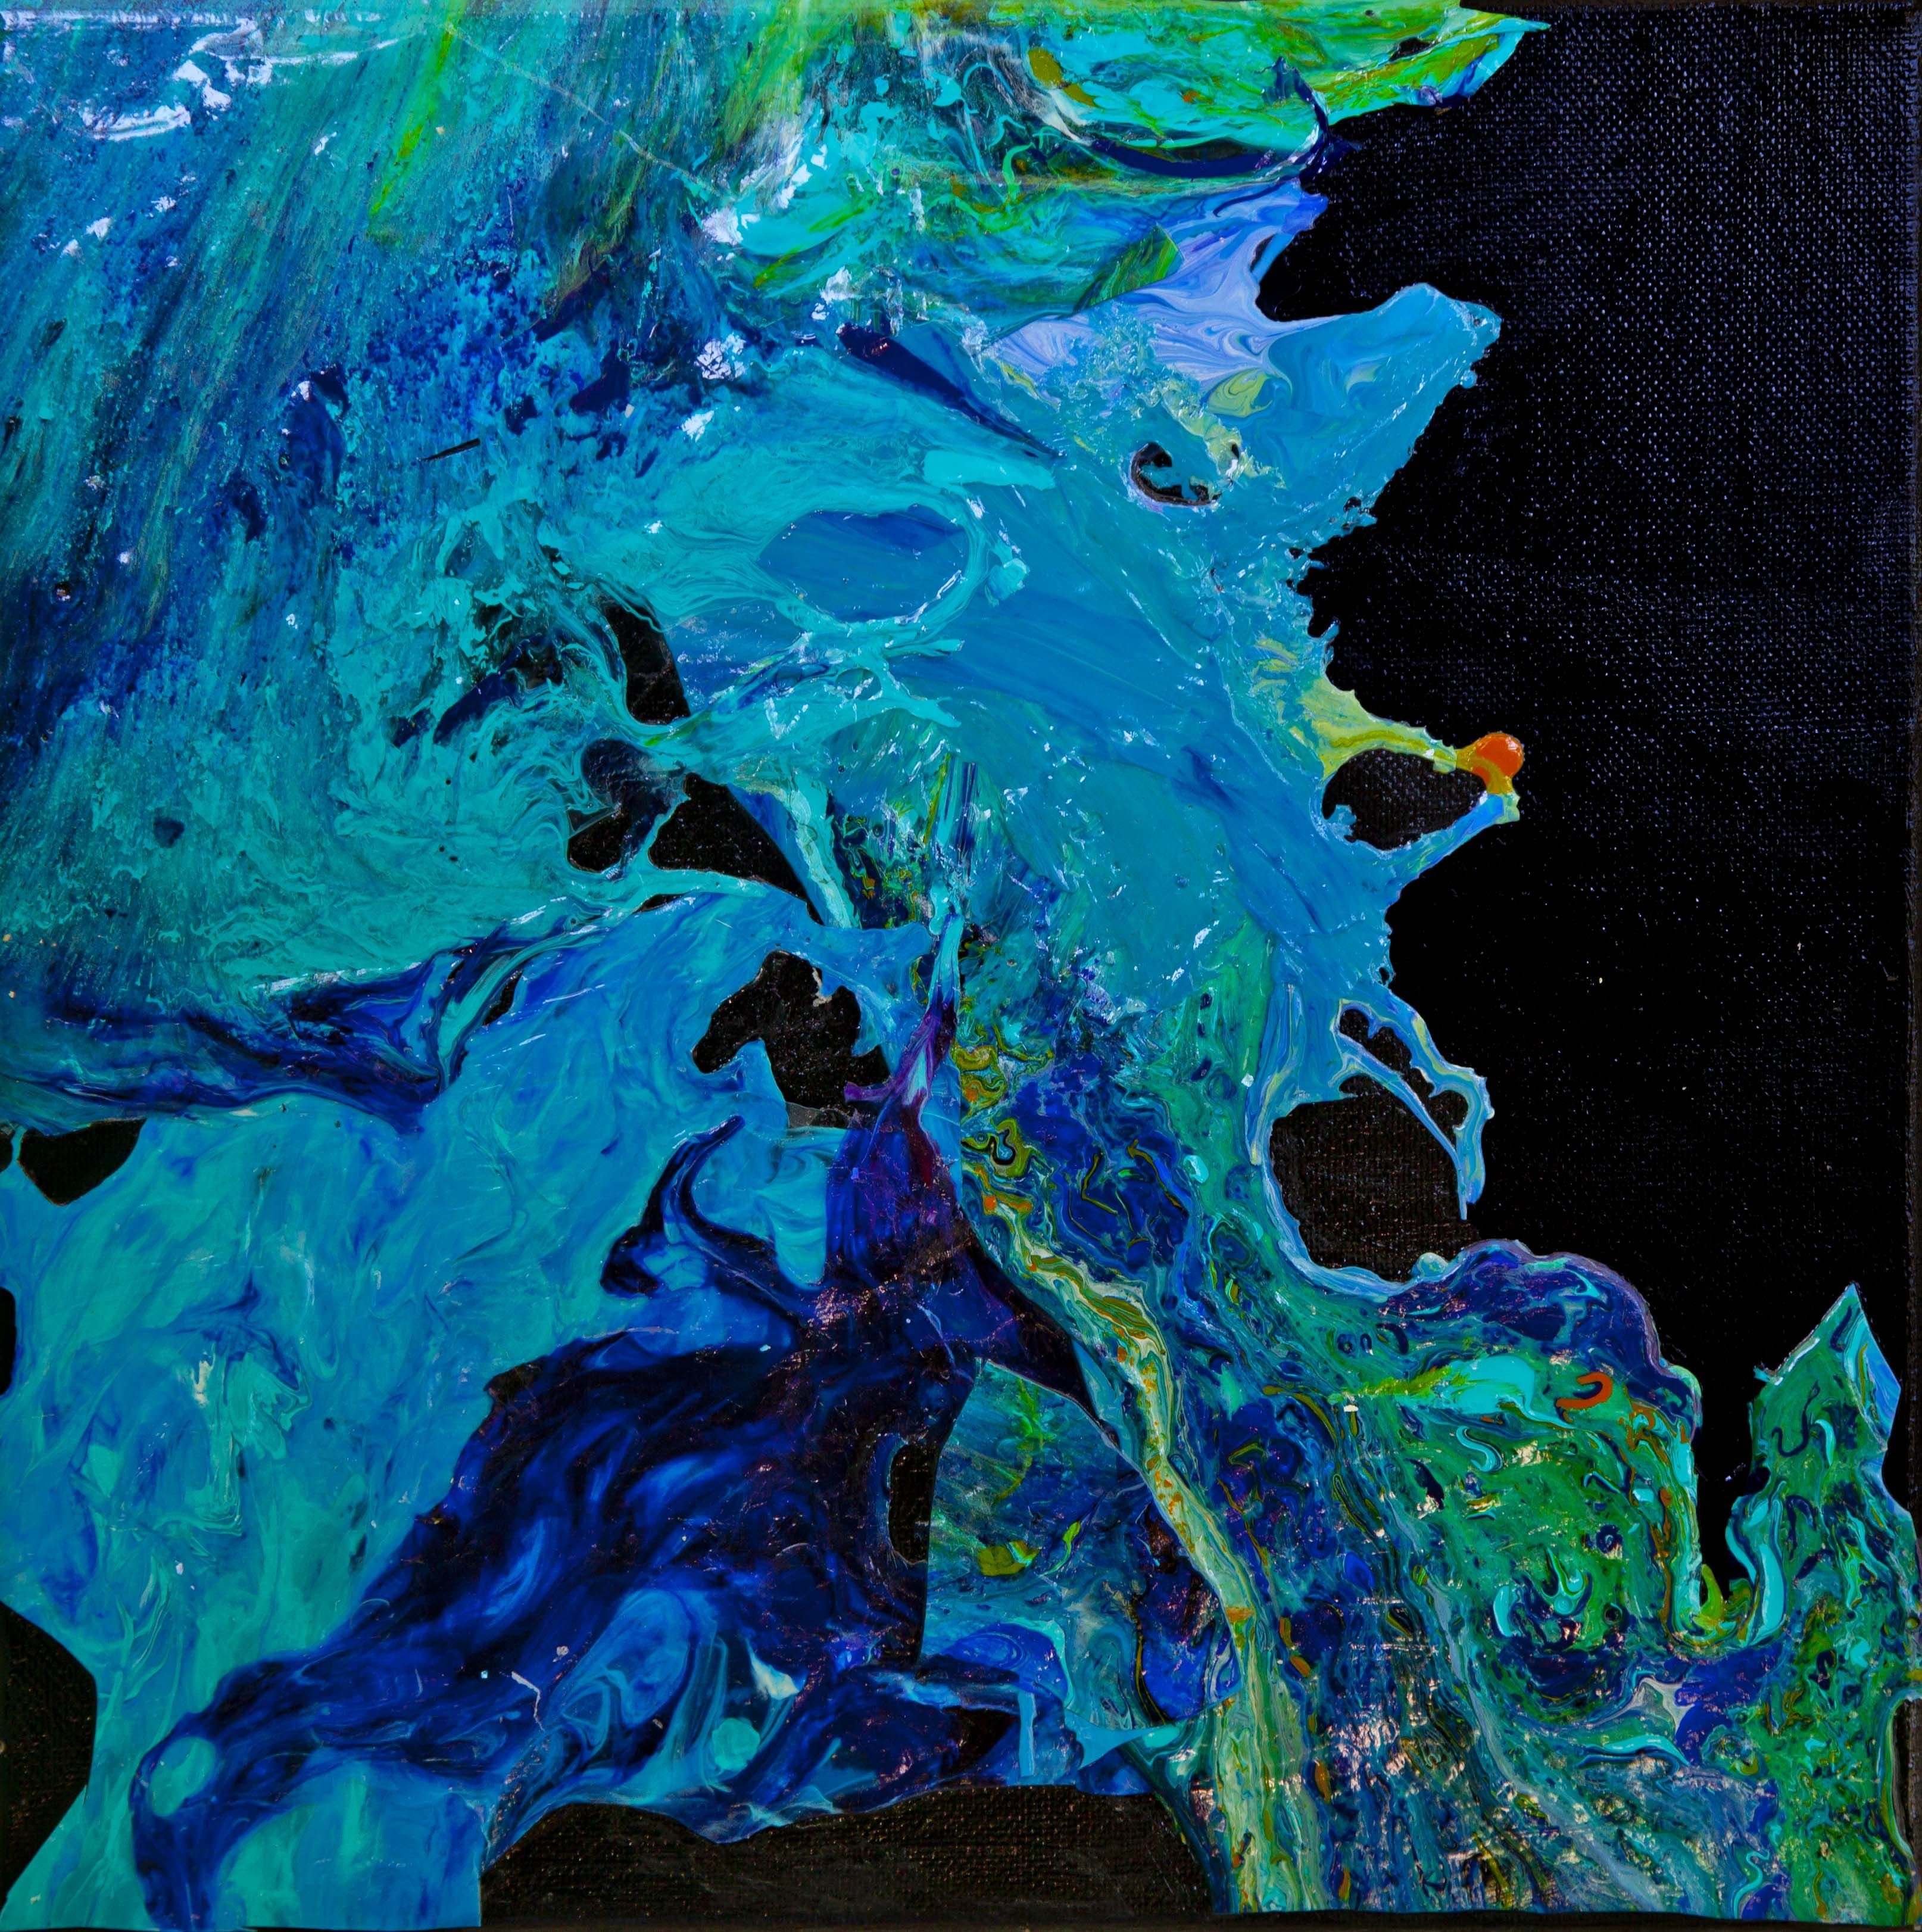
\includegraphics[width=1\linewidth]{graphics/1.jpg}
	%\end{figure}
%\end{frame}

\end{document}
